\section{Results} \label{Results}
At the time of this paper, only a brief survey has been conducted on a very early prototype of Karma History. We were only able to test an early prototype of our game which had about 5 minutes of content. Since we focused on generating different content both randomly and based on the player's choices we had each player play through our prototype twice. We noticed that players would spend a significant amount of time on the pre-game segment. Most players would pick the "good guys" faction of the world we represented in our prototype. The next phase would have a different location and character depending on the faction they picked. The next events could have varying numbers of choices for the player to pick depending on their choices in the earlier segments. This might not have been obvious to the players unless they were paying careful attention during their next playthrough. Unfortunately, a large portion of our testers experienced bugs or crashes that affected the overall quality of the session.
\par
After playing the game, each player was asked to take a short survey. The survey contained some short answer sections as well as sections asking a player to rate a value from 1 to 5. The key features we wanted each user to rate was, "Is the game creative?", "Does the generated story make sense?", and "Was the generated story varied?".

\begin{figure}[ht]
    \centering
    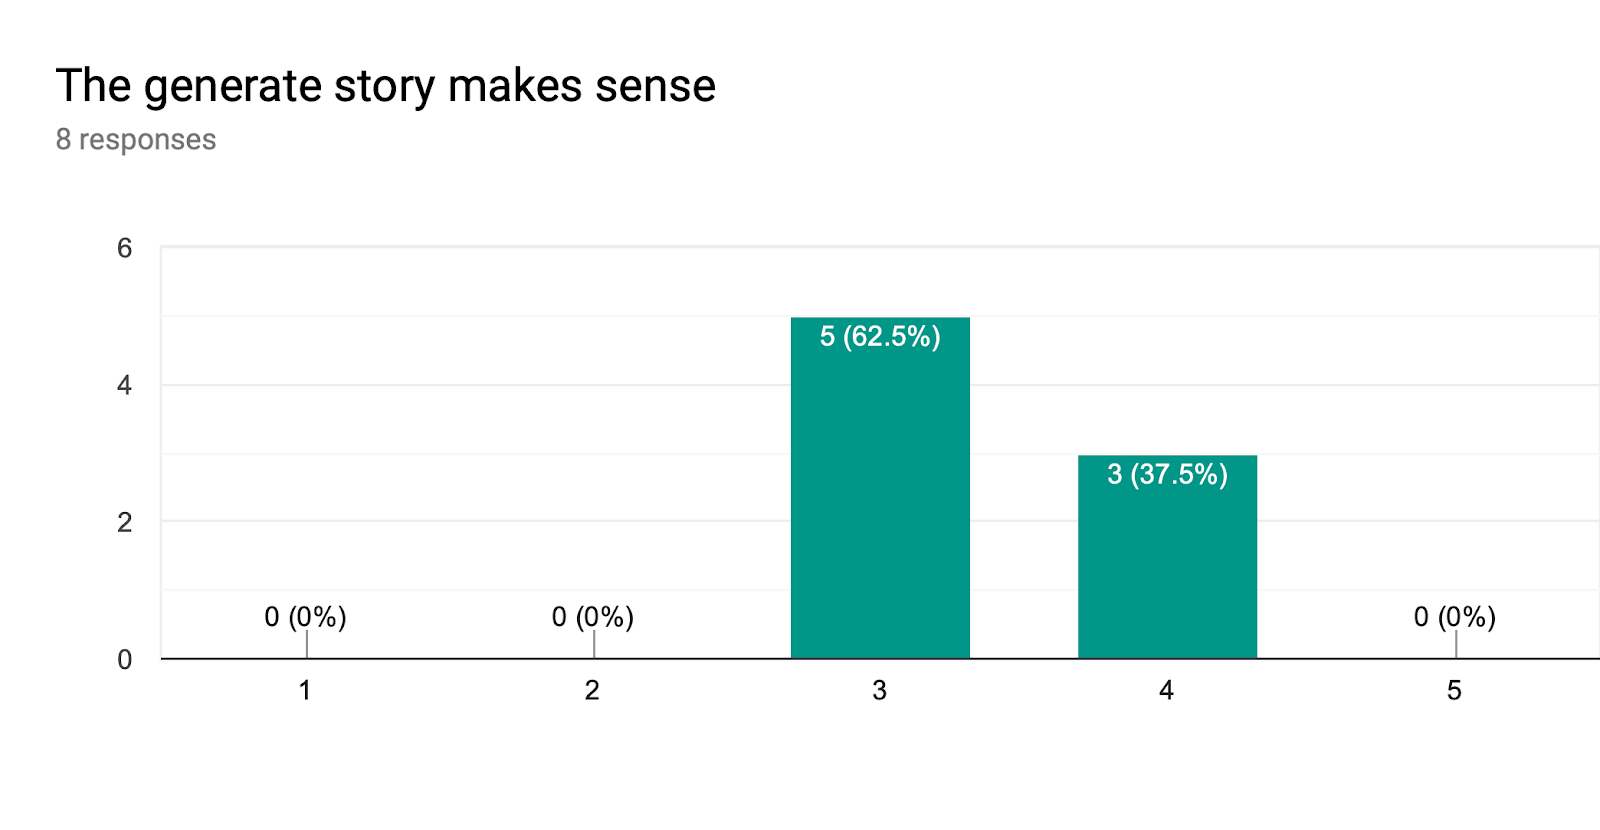
\includegraphics[width=0.3\textwidth]{images/s1.png}
    \caption{Survey: makes sense}
    \label{fig:s1}
\end{figure}

The results to "Is the game creative" were slightly positive but mostly neutral. As seen in \ref{fig:s2} the majority of users answered with either a 3 or 4. The results for "Does the generated story make sense?" \ref{fig:s1} and "Was the generated story varied" \ref{fig:s3} were similar. The results hint that our prototype showed some of these aspects, but not to a strong degree.

\begin{figure}[ht]
    \centering
    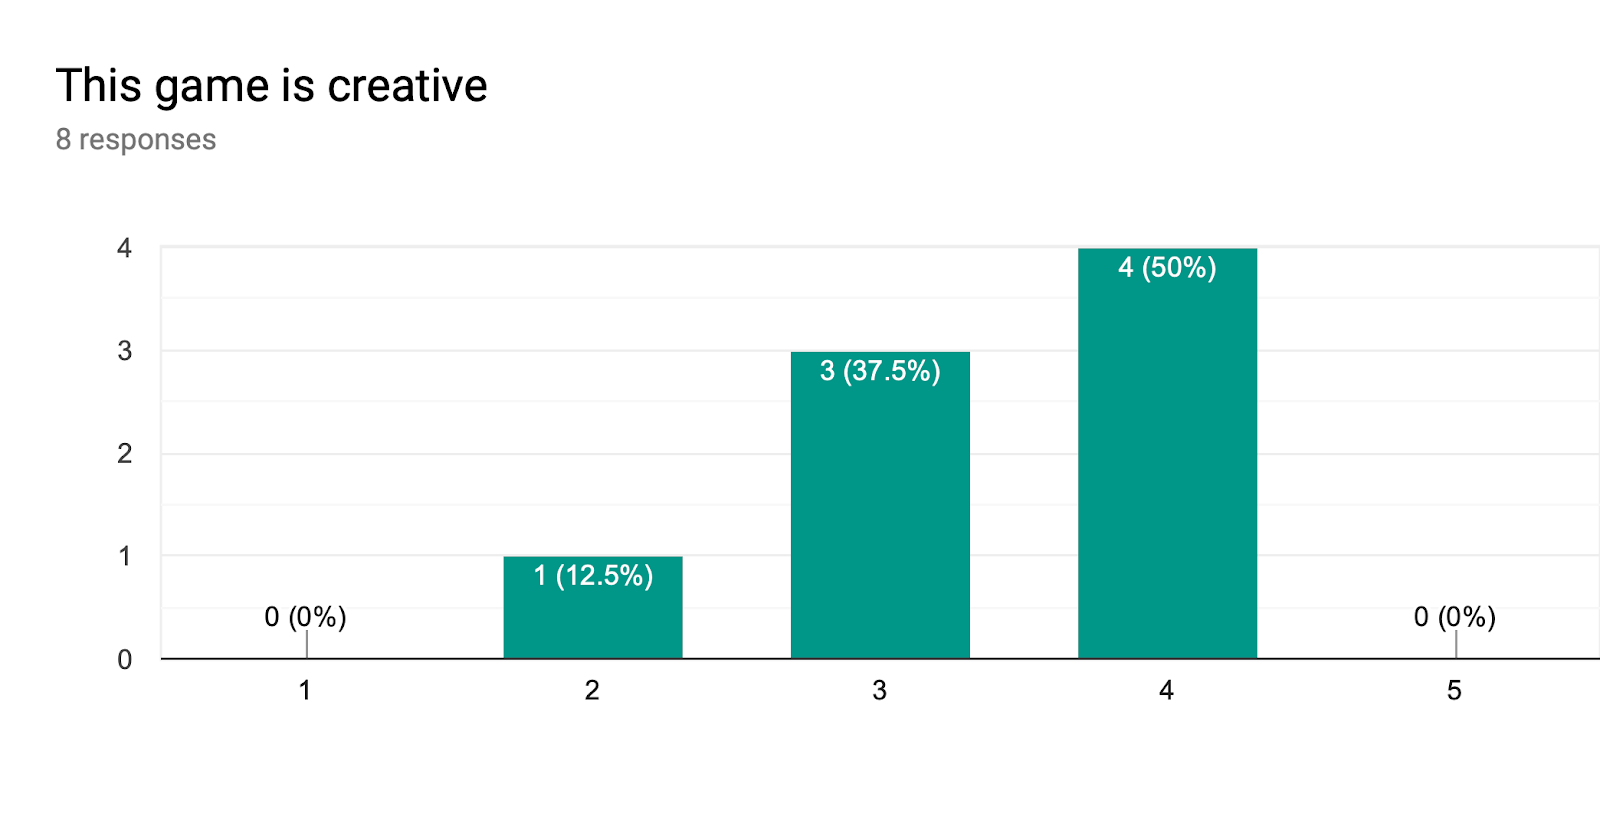
\includegraphics[width=0.3\textwidth]{images/s2.png}
    \caption{survey: is creative}
    \label{fig:s2}
\end{figure}

\begin{figure}[ht]
    \centering
    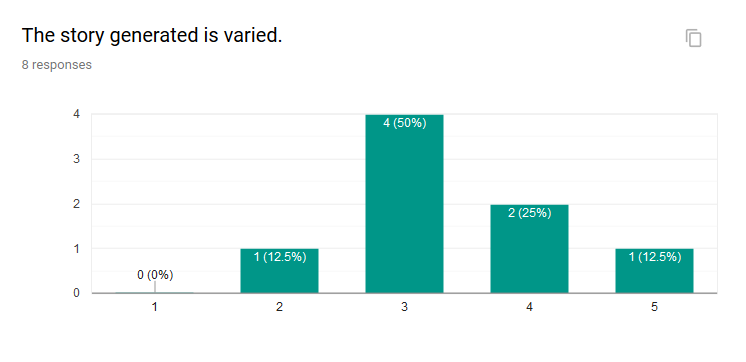
\includegraphics[width=0.3\textwidth]{images/s3.png}
    \caption{survey: story generation is varied}
    \label{fig:s3}
\end{figure}